\documentclass[10pt,twocolumn,letterpaper]{article}

\usepackage{cvpr}
\usepackage{times}
\usepackage{epsfig}
\usepackage{graphicx}
\usepackage{amsmath}
\usepackage{amssymb}
\usepackage{enumitem}

% Include other packages here, before hyperref.

% If you comment hyperref and then uncomment it, you should delete
% egpaper.aux before re-running latex.  (Or just hit 'q' on the first latex
% run, let it finish, and you should be clear).
\usepackage[breaklinks=true,bookmarks=false]{hyperref}

\cvprfinalcopy % *** Uncomment this line for the final submission

\def\cvprPaperID{****} % *** Enter the CVPR Paper ID here
\def\httilde{\mbox{\tt\raisebox{-.5ex}{\symbol{126}}}}

% Pages are numbered in submission mode, and unnumbered in camera-ready
%\ifcvprfinal\pagestyle{empty}\fi
\setcounter{page}{1}
\begin{document}

%%%%%%%%% TITLE
\title{Traffic-sign recognition system based on YOLO object detector and multi-class classifier}

\author{Lorenzo Busin\\
{\tt\small lorenzo.busin@gmail.com}
% For a paper whose authors are all at the same institution,
% omit the following lines up until the closing ``}''.
% Additional authors and addresses can be added with ``\and'',
% just like the second author.
% To save space, use either the email address or home page, not both
\and
Nicolò Tartaggia\\
{\tt\small nicolo.tartaggia@gmail.com}
}

\maketitle
%\thispagestyle{empty}

%\let\clearpage\relax
%% SEZIONI DEL DOCUMENTO
% qui vanno presentate in ordine di apparizione le sezioni che compongono il documento
\input{Res/Sezioni/Introduzione.tex}


%-------------------------------------------------------------------------
%%%%%%%%% ABSTRACT
\begin{abstract}
	The aim of the project is to build a traffic signs recognition system (TSRS) able to recognize different types of traffic signs. The task is similar to the built-in computer of modern cars, in fact those systems are capable to read traffic signs and to show important information to the driver improving his safety, such as traffic conditions, road rights, forbidden and allowed behaviors.
	The system is based on convolutional neural networks, a specific neural network particularly suitable for the areas of image detection and image classification.
	The main focus of this project is, firstly, to analyze the input image to detect potential traffic signs and, secondly, to classify each detected object via a multi-class classifier. In addition to this, we have expanded the functionality of this project to make it works even with video clips, so that the recognition of traffic signs takes place in real time. In order to explore the field of traffic sign recognition we adopt the YOLO object detection framework for detection and feature extraction processes together with a classification system based on Keras. Experimental results have demonstrated the effectiveness of the proposed system in terms of execution time and accuracy. 
\end{abstract}
%-------------------------------------------------------------------------
\section{Introduction}
Nowadays modern vehicles are usually equipped with powerful computers able to read and process data from sensors and cameras. In order to be able to provide the driver useful information fast enough, they should process data also in real time. With the birth and growth of intelligent systems, computer vision is increasingly used in the field of intelligent transport, which includes the subject of this paper: traffic sign recognition. It can be seen as a third eye which concerns a wide area of usages such as advanced driver assisting systems, autonomous driving and vehicle navigations. Other applications are system road surveying, building and maintaining maps of signs, mobile mapping systems, surveillance and self-govern robot navigation systems. These systems are typically based on detecting a region of interest (ROI), in which the traffic sign is located, recognizing typical characteristics such as color and geometric form. These information provide crucial visual details in order to understand the proper driving conditions. For example, they inform about speed limits, drivable lanes, obstacles, temporary situations, roadway access, restrictive areas, etc. Reasons why they are designed to be easily detectable, recognizable and interpretable by humans.
\begin{figure}[h]
	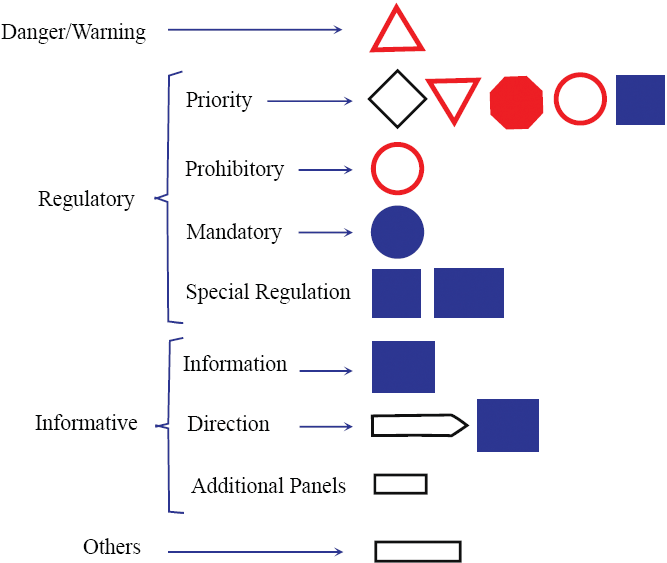
\includegraphics[width=\linewidth]{Res/Immagini/european-traffic-signs.PNG}	
	\caption{European Traffic Sign Categories}
\end{figure}

The application developed includes not only the standard functionality of image processing but also image and video detection and image classification. The idea is to concatenate different processes in order to compute the final labels for each traffic-sign without requiring a big amount of resources. In fact, traffic-sign detectors for large numbers of categories remains a challenging problem.\\ The process starts with the detection stage for the input image or video. This phase exploits the YOLO \cite{yolo} library for object detection which detects the area where a possible traffic sign is located and draws the so-called bounding boxes around it. We chose YOLO because of its main feature of being significantly faster than other framework, trading a bit of accuracy. Once the first step is completed, each object is passed to the classifier which is in charge to find out the correct label for the image. For this purpose we lean on Keras, a deep-learning framework which offers intuitive APIs and fits well for our project.  
%------------------------------------------------------------------------
\section{Related Work}
The idea behind this project is the development of an object recognition system. The term recognition refers to a suite of challenging computer vision tasks which can be divided into three categories:
\begin{itemize}[noitemsep,topsep=0pt]
	\item\textbf{Image classification}: predict the type or class of an object in an image;
	\item\textbf{Object localization}: locate the presence of objects in an image and indicate their location with a bounding box;
	\item\textbf{Object detection}: locate the presence of objects with a bounding box and types or classes of the located objects in an image.
\end{itemize}
In the last few years many application have been developed to explore different scenarios of object recognition through different techniques and deep learning models specifically dedicated \cite{wangMethods, tsrWithCnn, tsrWithCnn2}. Moreover with the continuous improvement of computing power available for the user, great progress has been made in the field of general object detection. The large amount of online projects and papers demonstrate how this field is growing year after year.\\
Our application aims to contribute to the traffic sign recognition problem, exploring the latest approaches of object detection and image classification. Here we present some published works related to our project. Also, readers are referred to the following survey for more details \cite{tsr20}.

\subsection{Traditional methods}
Traditional traffic sign detection methods can be summarized in color-based methods and shape-based methods. This phase includes image preprocessing, enhancement and segmentation according to the base attributes of color and shape. Given an image, the goal is to detect potential pixel areas which is the region of interest where an object may be located. Then the potential traffic sign is normalized in order to enter the classification phase.\\
Creusen et al. \cite{CreusenHog} propose a system based on Histogram of Oriented Gradients (HOG) algorithm. Using the color and shape informations they show that system performances improves because the gradient is less dependent on the background contents. Wang et al. \cite{WangRGB} try to reduce the impact of lightning conditions with a RGB normalization process. These methods, among others similar ones, suffer the environment features of the image. Anyway, they reach significant results.\\
For the classification purpose, researchers leaned on different machine learning algorithms. Support vector machine (SVM) is the most popular one \cite{soendoroSVM, greenSVM, rashidSVM}.

\subsection{CNN-based methods}
With the development of deep learning algorithms, the convolutional neural network (CNN) brings very good results. CNNs improve validation accuracy and robustness and reduce the requirements of quality of images and related computation. Qiao et al. \cite{qiaoCNN} proposed a system based on faster R-CNN to achieve region proposal, feature extraction and classification, which greatly reduces the repetitive computation and speeds up the operation. Mehta et al. \cite{mehtaCNN} compared different approach to regularize overfitting and showed that Adam optimizer adapts faster than other ones like Stochastic Gradient Descent (SGD). Kong et al. \cite{kongCNN} contributed with a lightweight cascaded CNN approach based on YOLO v2-tiny which reduced hardware complexity by decreasing the number of parameters.
Wang et al. \cite{wangCNN} explored CNN area including an accurate preprocessing stage to improve quality of the images.
%------------------------------------------------------------------------
\section{Dataset}
In this section we present the datasets we have used: one for the detection task and one for the classifier models. 
\subsection{Dataset for the detector}
For training the detector model using the YOLO algorithm, we built our own dataset. Firstly, we extracted a hundred JPG images from the DFG Traffic Sign Dataset\footnote{\url{http://www.vicos.si/Downloads/DFGTSD}} which consists of about 7000 images with 1920x1080 resolution captured in Slovenian roads. The RGB images were acquired with a camera mounted on a vehicle that was driven through six different Slovenian municipalities. The image data was acquired in rural as well as urban areas. Each image contains at least one traffic sign. After that, using a utility tool we manually selected for each image the coordinates of the position where the traffic signs are located. In such way, for each image in the training set there is a .txt file that indicates in each row the position of the traffic signs. To locate target objects we used the YOLO bounding box format (0, x-top left, y-top left, width, height) where 0 represents the class of the object (the model has only to detect the traffic signs location), x and y represent the coordinates of the top left corner, width and height represent the object dimensions. For testing this model we've taken other images from the same dataset. The same was done to build the validation set.


\subsection{Dataset for the classifier}
The Belgium Traffic Sign Dataset\footnote{\url{https://btsd.ethz.ch/shareddata}} refers to a set of 62 classes of traffic signs: training data files are divided into 62 folders that contain the images in PPM format. The same for validation data. We decided to cut some classes and to add some new ones in order to build an accurate classifier which focuses on most meaningful traffic signs. For some classes the number of images was too low to obtain a good result, so we merged this dataset with some images taken from the German Traffic Sign Recognition Benchmark\footnote{\url{http://benchmark.ini.rub.de}}, a dataset made for a multi-class image classification benchmark in the domain of advanced driver assistance systems and autonomous driving. The dataset we have used to train and to validate the classifier model is made of 56 traffic sign classes with 6229 images for training and 2493 for the validation. Every image is a cropped portion taken from a road picture which represents one traffic sign. Typically the images are characterized by small square sizes. The aim of the classifier is to pick the right class for each input image, but in Europe there could be small appearance differences between the same traffic sign classes from a country to another. 
\begin{figure}{}
	\centering
	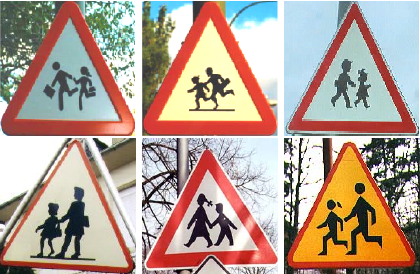
\includegraphics[width=0.6\linewidth]{Res/Immagini/differences.png}
	\caption{Differences between signs of the same class}\label{}
\end{figure}
To fix this issue, we manually added some images to training and validation data for classes which suffer this problem. Also, we adopted the augmentation technique to build a more generalized dataset and to prevent the overfitting problem. We added small variations to the input images introducing rotation by 10\%, width and height resizing, shearing and zooming randomly up to a tenth. It is important to not exaggerate with the changes because it could cause problems with the classification, due to the fact that some signs have specific orientation.

\subsection{Custom made test dataset}
The application is supposed to work in real-time situations and for this reason we recorded some videos using a front car camera. For video recording we have used an iPhone XR setting the quality on 1080p and 30 fps. We've taken short videos, from 30 seconds to a minute, for testing how good the combination of the detector and the classifier works.
%-------------------------------------------------------------------------
\section{Method}
Our method is composed of two consecutive operations: detection and classification. For the first one we adopted YOLO, an one-stage detector based on CNNs able to predict bounding boxes from input images directly without a region proposal step, achieving time efficiency and high inference speed. Therefore, it can be used not only for image detection but also for real-time devices. For the latter we built a multi-class classifier which receives as input the object detected. The reason why we don't adopt YOLO for the whole process is linked to the fact that there is a large number of classes to which a traffic sign could belong. Build a network capable of execute both detection and recognition requires a very long training time and one or more accurate and deep datasets.\\ 
One significant aspect that contributed to the choice of YOLO is the fact that it is a young framework constantly updated and supported by its team. In fact, the version used for this project is YOLOv3 \cite{yolov3}, released in 2018. The latest version, YOLOv4 \cite{yolov4}, was published on April 2020 but the lack of papers and projects to compare our results with lead us to choose the v3. 

\subsection{YOLO network setup}
To execute detection we setup the YOLO network in order to make it works with traffic signs and performs feature extraction. Its structure is composed of 53 convolutional layers with some shortcut connections which create a much more powerful network than the one used for the previous version YOLOv2. Despite being a bigger and deeper network, it is still more efficient than ResNet-101 or ResNet-152. Following this configuration the network has been pre-trained with a custom dataset. This process took many hours and produced a set of weights which, afterwards, have been given as input to build the correct network. For this purpose we use OperCV's \texttt{readNet} method. We also refer readers to explore YOLOv3 wiki\footnote{\url{https://github.com/AlexeyAB/darknet/wiki}} for its configuration and its weights. We also tried to setup the detector with a faster and smaller architecture called tiny-YOLO \cite{tinyYolo} whose performances are described in the next section.
\begin{figure}[h]
	\centering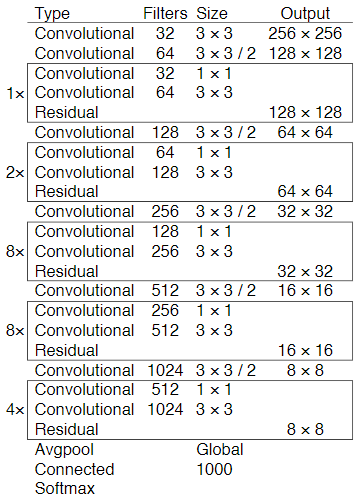
\includegraphics[scale=0.7]{Res/Immagini/darknet53.PNG}	
	\caption{Yolov3 structure (Darknet-53)}
\end{figure}

\subsection{YOLO algorithm}
%\begin{figure}[h]
%	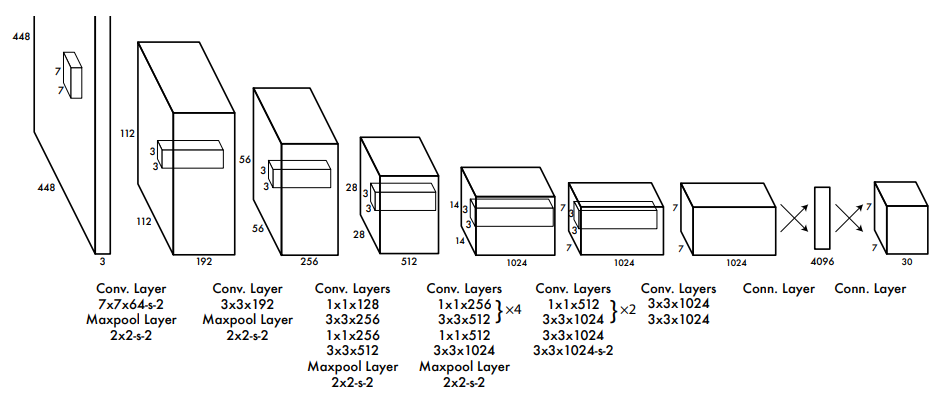
\includegraphics[width=\linewidth]{Res/Immagini/yoloArch.PNG}	
%	\caption{YOLO architecture}
%\end{figure}
The algorithm divides the input image into a $S$x$S$ grid. Each cell predicts the location of B bounding boxes, a confidence score and a probability of object class conditioned on the existence of an object in the bounding box. 
\begin{figure}[h]
	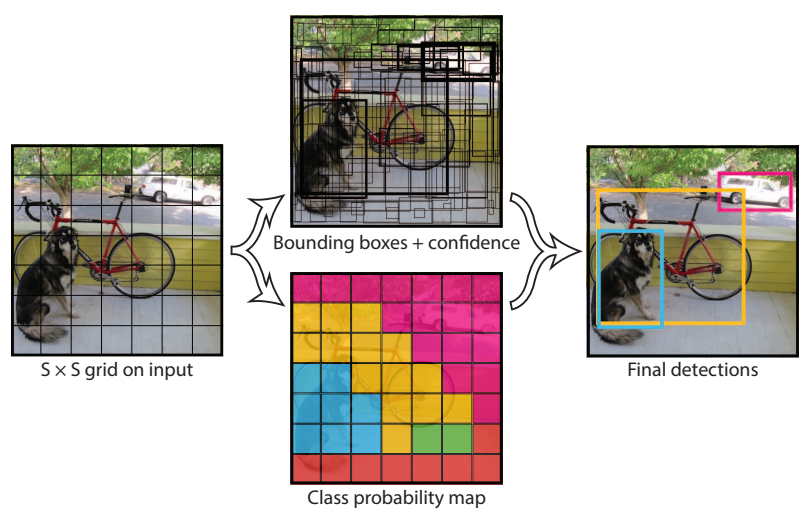
\includegraphics[width=\linewidth]{Res/Immagini/yoloAlg.PNG}	
	\caption{Workflow of YOLO}
\end{figure}
At training time one predictor is responsible for predicting an object based on which prediction has the highest current IOU (Intersection Over Union) with the ground truth. This leads to specialization between the bounding box predictors. Each predictor gets better at predicting certain sizes, aspect ratios, or classes of object, improving overall recall.\\
After that, each traffic sing is extracted, cropping the original image through coordinates of its predicted bounding box, and passed as input to the classifier. Image detection and real-time detection can be performed using respectively \texttt{image\_analysis} method and \texttt{video\_analysis} method.

\subsection{Classification}
Our classification process is based on Keras\footnote{\url{https://keras.io/}}. In particular, we rely on Keras sequential model. It allows us to create models layer by layer in a step by step fashion. Keras provides also another type of model: the functional model. It is flexible as each layer can be connected in a pairwise fashion and can create complex networks. Since this was our first approach, we built and trained different convolutional neural networks through the sequential procedure which was easier to implement; nevertheless the results we gained are satisfying.\\
Our reference model called CNN3 is composed of 26 layers. The structure of the first 6 ones is repeated 3 times: two consecutive 2D convolutional layers with ReLu activation function each and $3$x$3$ kernel size, a layer for 2D max pooling operation and finally a layer for the dropout. The inputs are then flattened and pass through some dense layers. The other models, CNN1 and CNN2, are a simplified version of CNN3. We also implemented the LeNet architecture to test our classifier with a known convolutional neural network and to compare our experiments.\\
The classifier is built with Keras \texttt{load\_model} method and is used to compute the final label for the input image and its associated probability.
\begin{figure}[h]
	\centering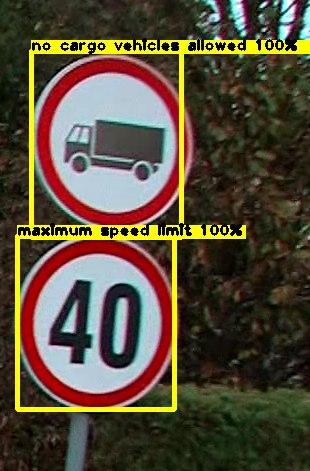
\includegraphics[scale=0.5]{Res/Immagini/classExample.jpg}	
	\caption{Final output}
\end{figure}
%------------------------------------------------------------------------
\section{Experiments}
Initially we trained the models and tested them independently using the validation sets for the classifiers and for the detectors. After that, we proceeded to manually testing the 2 step detection and classification technique, analyzing both images and videos in different scenarios. 


\subsection{Detection models}
We trained the detector models on Google Colab with 2 CPUs Intel Xeon @ 2.30 GHz, 13 GB of RAM and Nvidia Tesla K80 GPU. The YOLO model was trained for 4000 epochs with 64 batch size and it took about 24 hours and the tiny-YOLO model was trained for 4000 epoch with 64 batch size and it took about 4 hours.
For training  the models we used convolutional weights that are pre-trained on ImageNet model\footnote{\url{https://pjreddie.com/darknet/imagenet}}. Pre-trained weights was used as initializers for the new training procedures. This technique is also called transfer learning and avoids learning everything from scratch. The dataset used to compute this metric was the validation set manually built, as explained above. The computation of the accuracy value for a detection task is not trivial. We developed a specific method for this purpose. The main idea is that the detector selects with bounding boxes the position of the traffic signs, selecting the x and y coordinates of the top left corner, the width and the height of each sign, hence using the YOLO format as for the annotations which represented the ground-truth. So, we compared for each traffic signs one by one these values with 10\% of confidence: this value has been chosen considering the human error made during the dataset construction and a small prediction error. 
The results (see Table \ref{yolo-metrics}) show up a substantial difference between the accuracy values but also a substantial difference on the training times. This is due to the fact that tiny-YOLO is a lighter version of the YOLO model. In any case, considering a detection as a bad one doesn't mean that the detection is wrong, but only not well defined for that sign and consequently implies a higher probability of error for the classifier.


\subsection{Classification models}
We trained the classifier models with 4 CPUs Intel Core i7-6700HQ @ 2.6 GHz, 8 GB of RAM and Nvidia GeForce GTX 950M. All models were trained for 100 epochs with 16 batch size and they took different training times. The metrics values of each model were computed after their training using the validation set, as explained above. The results (see Table \ref{class-metrics}) show up that CNN1 has obtained the worst values because of its shallowness. The other models reached good and similar values, but CNN3 achieved the best performance.


\subsection{Detection with classification testing}
Analyzing the obtained results we selected the best combination of detector and classifier. As detector we had chosen the YOLO model because the detection task is fundamental for a good classification: in fact, for getting accurate predictions the bounding boxes have to be precise as possible. As classifier we had chosen the CNN3 model because it reached the best accuracy value with a reasonable training time. Testing automatically the fully working application was very difficult and for this reason we spent a lot of time for testing it manually. Initially, we tested the 2 step detection and classification for road images analysis and then we tested it for videos analysis. During the video analysis, in fact, each frame is processed independently like a single image. The dataset we used for the experiments is our custom made dataset, as above explained. We also compared the same road in different light conditions, like day and night. During the day, the detector is able to spot traffic signs from a long range and hence to classify them. During the night, instead, signs can be spotted only at close range: the detection distance can be increased if the road is provided by street lamps which light up the signs enough for their identification. 
The difficulty of this task is the variety of different scenarios that we have to face on road. According with Serna et al. \cite{gamezPaper} results, we found that most of the misclassified traffic signs show the following characteristics:
\begin{itemize}[noitemsep,topsep=0pt]
	\item Bad lighting;
	\item Strong motion blur;
	\item Human added artifacts;
	\item Poor image quality;
	\item Strong shadows or highlights;
	\item Occlusions;
	\item Strong similarity with other signs.
\end{itemize} 
All of the elements listed above are commonly found on the roads and all of them contribute to the increase of the probability of error.

\begin{table}[h!]
	\begin{center}
		\begin{tabular}{|c|c|c|}
			\hline
			Model & Accuracy & Training time (h) \\
			\hline\hline
			YOLO & 0.97 & 24 \\
			tiny-YOLO & 0.84 & 4 \\
			\hline
		\end{tabular}
	\end{center}
	\caption{Metrics for detection models}
	\label{yolo-metrics}
\end{table}

\begin{table}[h!]
	\begin{center}
		\begin{tabular}{|c|c|c|c|c|}
			\hline
			Model & Accuracy & Precision & Recall & Training time (m) \\
			\hline\hline
			CNN1 & 0.86 & 0.88 & 0.83 & 11 \\
			CNN2 & 0.95 & 0.96 & 0.96 & 41 \\
			CNN3 & 0.96 & 0.96 & 0.95 & 23 \\
			LeNet & 0.92 & 0.93 & 0.90 & 12 \\
			\hline
		\end{tabular}
	\end{center}
	\caption{Metrics for classification models}
	\label{class-metrics}
\end{table}
%-------------------------------------------------------------------------
\section{Conclusion}
We proposed a solution for the detection and the classification of European traffic signs. We explored the world of autonomous vehicles, a new and growing topic. We adopted the modern state-of-the-art YOLO algorithm to build a fast object detection system, but it also isn't always very accurate like other CNN based systems which focus a lot on the objects to detect but at the same time are much slower. This work is very complex due to the different factors that can influence the detection or the classification.

The strengths of our system are extensibility and modularity. We introduced a 2 step detection and classification model, this means that the detection task and the classification task are independent from each other. One could change a model without modifying the other or changing the system's architecture. It is also possible to easily extend the number of classes of the classifier.

The drafting of this paper helped us to understand and to exercise on finding new solutions and carrying out experiments quickly, establishing metrics for their evaluation and comparison. The operation that took the longest time was the training of models and that made more difficult trying out new ideas or experiments. We learned the state-of-the-art YOLO algorithm for object detection, making use of methods from the libraries OpenCV and Keras. We also experienced how to deal with papers extracting valuable information and applying it in our work.

In future work we intent to:
\begin{itemize}[noitemsep,topsep=0pt]
	\item Test the model using the newest YOLOv4, the recent release of the fourth version of YOLO algorithm which should offers better performance;
	\item Expand the dataset including new traffic sign classes or expanding classes already present like speed limit signals in order to build a more precise model;
	\item Add images for that classes which suffer the problem of intra-class appearance differences;
	\item Use custom loss function to obtain more accurate detections;
	\item Try different data augmentation settings to improve the classifier accuracy, for example introducing photo-metric distortions like changing the brightness, saturation, contrast and noise or trying other interesting techniques of augmenting the images like CutOut \cite{cutout} which randomly masks out square regions of input during training  or Random Erasing \cite{random} which selects rectangle regions in an image and erases its pixels with random values, in order to improve robustness and performance of CNNs;
	\item Try to implement the classifier through a functional model using the Keras functional API \footnote{\url{https://keras.io/guides/functional_api}}  which is a way to create models that are more flexible than the Sequential API. In fact, can handle models with non-linear topology, shared layers, and even multiple inputs or outputs in order to build graphs of layers.
\end{itemize}
%-------------------------------------------------------------------------


\begin{thebibliography}{9}
	
	\bibitem{yolo}
		J. Redmon, S. Divvala, R. Girshick, and A. Farhadi, “You only look
		once: Unified, real-time object detection”. In \textit{2016 IEEE Conference on Computer Vision and Pattern Recognition (CVPR)}, pp. 779–788, June
		2016.
	
	\bibitem{wangMethods}
		C. Wang, "Research and Application of Traffic Sign Detection and Recognition Based on Deep Learning". In \textit{2018 International Conference on Robots \& Intelligent System (ICRIS)}, Changsha, pp. 150-152. DOI: 10.1109/ICRIS.2018.00047.
	
	\bibitem{tsrWithCnn}
		Y. Sun, P. Ge and D. Liu, "Traffic Sign Detection and Recognition Based on Convolutional Neural Network". In \textit{2019 Chinese Automation Congress (CAC)}, Hangzhou, China, pp. 2851-2854. DOI: 10.1109/CAC48633.2019.8997240.
		
	\bibitem{tsrWithCnn2}
		D. Tabernik and D. Skočaj, "Deep Learning for Large-Scale Traffic-Sign Detection and Recognition". In \textit{April 2020 IEEE Transactions on Intelligent Transportation Systems} vol. 21, no. 4, pp. 1427-1440. DOI: 10.1109/TITS.2019.2913588.
	
	\bibitem{tsr20}
		B. Sanyal, R. K. Mohapatra and R. Dash, "Traffic Sign Recognition: A Survey". In \textit{2020 International Conference on Artificial Intelligence and Signal Processing (AISP)}, Amaravati, India, pp. 1-6. DOI: 10.1109/AISP48273.2020.9072976.
		
	\bibitem{CreusenHog}
		 I.M. Creusen, R.OJ. Wijnhoven, E. Herbschleb, and P.H.N. de With, "Color exploitation in hog-based traffic sign detection". In  \textit{September 2010 Proc. of the IEEE International Conference on Image Processing (Ic/P)}, pp. 2669-2672. DOI: 10.1109/ICIP.2010.5651637.
		 
	\bibitem{WangRGB}
		Qiong Wang and X. Liu, "Traffic sign segmentation in natural scenes based on color and shape features". In \textit{2014 IEEE Workshop on Advanced Research and Technology in Industry Applications (WARTIA)}, Ottawa, ON, pp. 374-377. DOI: 10.1109/WARTIA.2014.6976273.
		
	\bibitem{soendoroSVM}
		D. Soendoro and I. Supriana, "Traffic sign recognition with Color-based Method, shape-arc estimation and SVM." In \textit{Proceedings of the 2011 International Conference on Electrical Engineering and Informatics} Bandung, pp. 1-6. DOI: 10.1109/ICEEI.2011.6021584.
		
	\bibitem{greenSVM}
		J. Greenhalgh and M. Mirmehdi, "Real-Time Detection and Recognition of Road Traffic Signs". In \textit{December 2012 IEEE Transactions on Intelligent Transportation Systems, vol. 13, no. 4}, pp. 1498-1506. DOI: 10.1109/TITS.2012.2208909.
		
	\bibitem{rashidSVM}
		S. I. Rashid, M. A. Islam and M. A. M. Hasan, "Traffic Sign Recognition by Integrating Convolutional Neural Network and Support Vector Machine". In  \textit{2019 International Conference on Computer, Communication, Chemical, Materials and Electronic Engineering (IC4ME2)}, Rajshahi, Bangladesh, pp. 1-6. DOI: 10.1109/IC4ME247184.2019.9036651.
	
	\bibitem{qiaoCNN}	
		K. Qiao, H. Gu, J. Liu and P. Liu, "Optimization of Traffic Sign Detection and Classification Based on Faster R-CNN". In \textit{2017 International Conference on Computer Technology, Electronics and Communication (ICCTEC)}, Dalian, China, pp. 608-611. DOI: 10.1109/ICCTEC.2017.00137.
		
	\bibitem{mehtaCNN}
		S. Mehta, C. Paunwala and B. Vaidya, "CNN based Traffic Sign Classification using Adam Optimizer". In \textit{2019 International Conference on Intelligent Computing and Control Systems (ICCS)}, Madurai, India, pp. 1293-1298. DOI: 10.1109/ICCS45141.2019.9065537.
		
	\bibitem{kongCNN}
	S. Kong, J. Park, S. Lee and S. Jang, "Lightweight Traffic Sign Recognition Algorithm based on Cascaded CNN," 2019 19th International Conference on Control, Automation and Systems (ICCAS), Jeju, Korea (South), 2019, pp. 506-509, doi: 10.23919/ICCAS47443.2019.8971735.
	
	\bibitem{wangCNN}
		J. Wang, W. Wang and A. Zhou, "The Faster Detection and Recognition of Traffic Signs Based on CNN". In \textit{2019 IEEE 14th International Conference on Intelligent Systems and Knowledge Engineering (ISKE)}, Dalian, China, pp. 907-914. DOI: 10.1109/ISKE47853.2019.9170338.
		
	\bibitem{gamezPaper}
		Gamez Serna, Citlalli and Ruichek, Yassine, 2018, \textit{Classification of Traffic Signs: The European Dataset}. IEEE Access. PP. 1-1. 10.1109/ACCESS.2018.2884826. 
		
	\bibitem{yolov3}
		Joseph Redmon, Ali Farhadi, "YOLOv3: An Incremental Improvement". 2018, \href{https://arxiv.org/abs/1804.02767}{arXiv:1804.02767 [cs.CV]}.
		
	\bibitem{yolov4}
		Alexey Bochkovskiy, Chien-Yao Wang and Hong-Yuan Mark Liao, "YOLOv4: Optimal Speed and Accuracy of Object Detection". 2020, \href{https://arxiv.org/abs/2004.10934}{arXiv:2004.10934 [cs.CV]}.
		
	\bibitem{tinyYolo}
		Rachel Huang, Jonathan Pedoeem and Cuixian Chen, "YOLO-LITE: A Real-Time Object Detection Algorithm Optimized for Non-GPU Computers". 2018, \href{https://arxiv.org/abs/1811.05588}{arXiv:1811.05588 [cs.CV]}
		
	\bibitem{cutout}
		Terrance DeVries and Graham W. Taylor, "Improved Regularization of Convolutional Neural Networks with Cutout". 2017,
		\href{https://arxiv.org/abs/1708.04552}{arXiv:1708.04552 [cs.CV]}
		
	\bibitem{random}
		Zhun Zhong and Liang Zheng and Guoliang Kang and Shaozi Li and Yi Yang, "Random Erasing Data Augmentation". 2017,
		\href{https://arxiv.org/abs/1708.04896}{arXiv:1708.04896 [cs.CV]}
	
\end{thebibliography}


%{\small
%\bibliographystyle{ieee_fullname}
%\bibliography{egbib}
%}

\end{document}
